\section{Exercise 11}
\subsection{}
Testing method(also for 11.b):
I let the the crawler walk until he disappears from the screen at the end.
That is one run. I measure the run time in ticks. I take 8 runs.
The runs are consecutive.

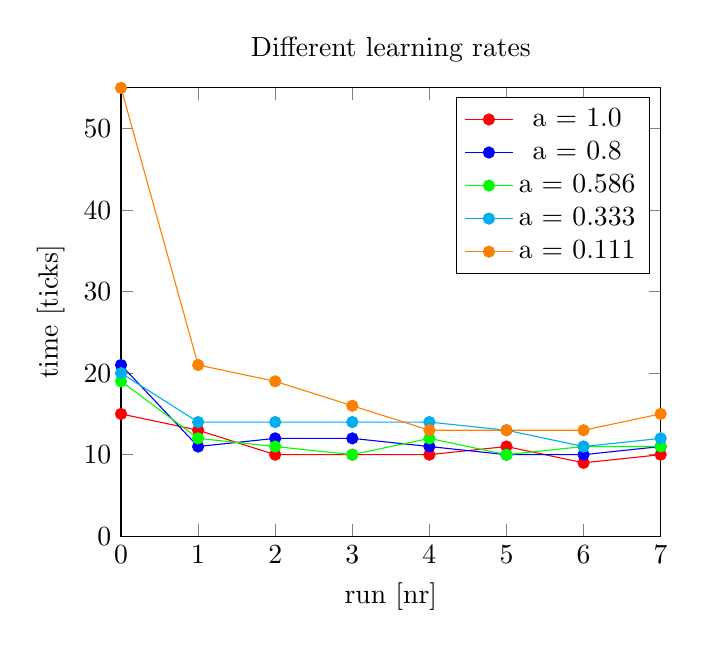
\begin{tikzpicture}
\begin{axis}[
    title={Different learning rates},
    xlabel={run [nr]},
    ylabel={time [ticks]},
    xmin = 0, xmax = 7,
    ymin = 0, ymax = 55
]
\addplot[
    color=red,
    mark=*
]
coordinates{(0,15)(1,13)(2,10)(3,10)(4,10)(5,11)(6,9)(7,10)};
\addplot[
    color=blue,
    mark=*
]
coordinates{(0,21)(1,11)(2,12)(3,12)(4,11)(5,10)(6,10)(7,11)};
\addplot[
    color=green,
    mark=*
]
coordinates{(0,19)(1,12)(2,11)(3,10)(4,12)(5,10)(6,11)(7,11)};
\addplot[
    color=cyan,
    mark=*
]
coordinates{(0,20)(1,14)(2,14)(3,14)(4,14)(5,13)(6,11)(7,12)};
\addplot[
    color=orange,
    mark=*
]
coordinates{(0,55)(1,21)(2,19)(3,16)(4,13)(5,13)(6,13)(7,15)};
\legend{a = 1.0, a = 0.8, a = 0.586, a = 0.333, a = 0.111}
\end{axis}
\end{tikzpicture}

\newpage{}
The higher the learningrate, the faster the crawler's policy 
converges. But, lower learningrate's do not slow the process of 
learning down much, till a certain point. After that the learning 
speed is affected significantly, as you can see with the orange line 
in the graph. Eventually they will converge, sooner or later. 

\subsection{}

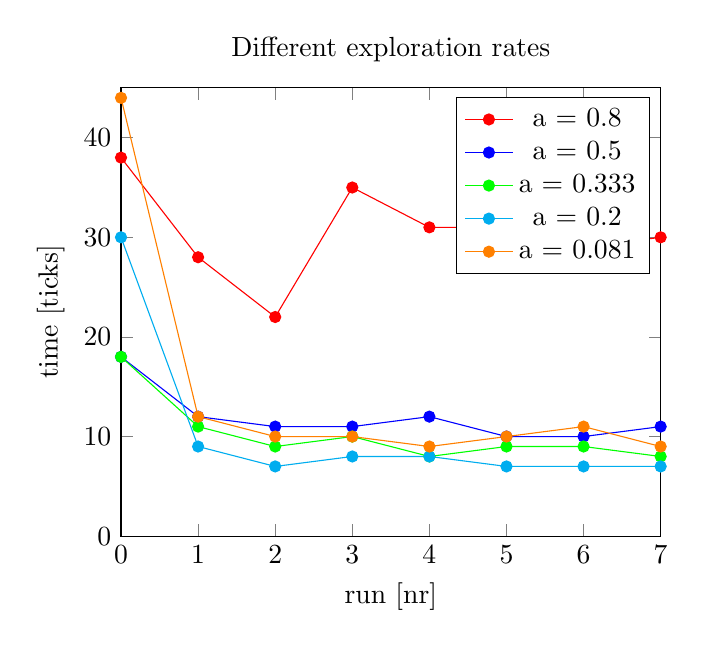
\begin{tikzpicture}
\begin{axis}[
    title={Different exploration rates},
    xlabel={run [nr]},
    ylabel={time [ticks]},
    xmin = 0, xmax = 7,
    ymin = 0, ymax = 45
]
\addplot[
    color=red,
    mark=*
]
coordinates{(0,38)(1,28)(2,22)(3,35)(4,31)(5,31)(6,29)(7,30)};
\addplot[
    color=blue,
    mark=*
]
coordinates{(0,18)(1,12)(2,11)(3,11)(4,12)(5,10)(6,10)(7,11)};
\addplot[
    color=green,
    mark=*
]
coordinates{(0,18)(1,11)(2,9)(3,10)(4,8)(5,9)(6,9)(7,8)};
\addplot[
    color=cyan,
    mark=*
]
coordinates{(0,30)(1,9)(2,7)(3,8)(4,8)(5,7)(6,7)(7,7)};
\addplot[
    color=orange,
    mark=*
]
coordinates{(0,44)(1,12)(2,10)(3,10)(4,9)(5,10)(6,11)(7,9)};
\legend{a = 0.8, a = 0.5, a = 0.333, a = 0.2, a = 0.081}
\end{axis}
\end{tikzpicture}

The exploration rate let the crawler take random actions to discover 
new things. A high exploration rate will never be fast. Even if the 
agent has tried many things and learned the optimal policy from it, 
it will still perform random actions instead of the learned ones. 
As you can see with the red line, the time of completion stays high. 
Lowering the exploration rate let the crawler move faster due to less 
random moves, but if we drop it to low it will learn less fast. We 
can see that lower rates do better, for all except the lowest value here.
We can see that the orange line is consistently above the cyan line, 
breaking the trend. Many more tests may reveal a optimal learning rate 
somewhere between cyan and orange.

\subsection{}

high a(learningrate), low e(explorationrate) = learns fast from actions performered, but tries little new things.
Since he does not know anything to start with, he needs to randomly come across a good action at the right time.
The low e value holds the crawler back from learning as fast as he could.

high a, high e = learns fast from actions performered, and also tries many things(random) out.
This combination lets the crawler learn rapidly at the beginning. However, when he has learned to walk, the high e
holds him back from performing at his best. Because a high e brings a high probability for a random action, his
behaviour is quite random. Now he knows the right actions, this is not needed anymore. Many steps are now wasted, the random
actions do not contribute walking faster and could even push him back at bit.

low a, low e = This is a very slow learning combination. There is a low chance that he will randomly do something.
And if he randomly does something right, it picks it up slow because of the low a. But when it, eventually, learned how to walk
he performs great. He will not disrupt his walk with randomness, and random bad actions do not influence him because of
the low a.

low a, high e = This one is weird. He tries many things, but learns from them slowly. When he learned to crawl, randomness
still disrupts his speed. But this time it will not affect the learned policy so much.

The best thing is to have a high e and a high a, so he learns fast. He will start walking in no time. Then you can decrease
the e and a slowly as he gets better. At the end set them to zero as the learning has finalised. Then there will be no
randomness to disrupt the crawl, and the crawler will be at his fastest.

\subsection{}

The learningrate has influence on how strong newly learned samples 
affect the agent, as it is a multiplier for the whole sample.
The discount value is a multiplier for only a part of the sample.
It makes the value in the next state less import for the value of the 
current state. The learningrate dictates how fast the agent adapts, 
the discount rate dictates how much the agent plans ahead. When you 
change the learningrate it changes how fast the policy converges and 
later on how stable the policy stays. But the crawler learns the same 
policy for different learningrate values: it moves in the same way 
after the policy is converged. This does not hold for the discountrate.
A different discountrate produces a different policy: the agent moves 
differently. A low discount rate will make the agent more focussed on 
the short term. He want to move forward in the moment. But if he looks 
ahead he could have seen that a better more effective movement is 
possible. It is clear when you try out a higher discount, the agent 
learns a better policy: the crawler moves faster! So does the effect 
of changing the learningrate depend on the discountrate? No, the effect 
of the learningrate still effects the way the policy converges the 
same, it just converges to a different policy.

\subsection{}

The good explorationrate let the agent do random actions to learn from.
It results in a better policy. The explorationrate and the discountrate
both affect the policy. The effect can look the same but there is a 
clear difference. With a low discountrate, a good explorationrate will 
help find a good shortterm policy. With a high discountrate, a good 
explorationrate will help find a good longterm policy. They might seem 
a bit more related to eachother than the case with the learningrate, 
but they do just like the learningrate really there own thing.